\begin{frame}
\frametitle{Разделение на большие и маленькие алокации}
\begin{itemize}
  \item До сих пор мы не учитывали никак сколько и зачем мы алоцируем память:
  \begin{itemize}
    \item часто нужно алоцировать память под объекты одного типа и,
    соответственно, размера;
    \item большие участки памяти алоцируются реже и живут, зачастую, долго;
  \end{itemize}
  \item Разобьем задачу на несколько более простых задач:
  \begin{enumerate}
    \item научимся эффективно алоцировать большие регионы памяти;
    \item научимся эффективно алоцировать регоны фиксированного размера.
  \end{enumerate} 
\end{itemize}
\end{frame}

\begin{frame}
\frametitle{Алокация больших регионов}
\begin{itemize}
  \item Будем алоцировать только регионы кратные некоторому размеру
  \emph{PAGE\_SIZE}:
  \begin{itemize}
    \item \emph{PAGE\_SIZE} выбирается исходя из задачи;
    \item например, \emph{PAGE\_SIZE} может быть 4Kb или около того;
  \end{itemize}
  \item не будем добавлять к аллоцированной памяти никаких заголовков и прочего:
  \begin{itemize}
    \item в отличие от предыдущего алгоритма в этом нет необходимости;
    \item мы всегда будем алоцировать столько, сколько запросили и пользователь
    сам может хранить размер;
  \end{itemize}
  \item алоцированные регионы всегда выровнены на границу \emph{PAGE\_SIZE}.
\end{itemize}
\end{frame}

\begin{frame}
\frametitle{Buddy Allocator}
\begin{itemize}
  \item Будем алоцировать блоки не просто кратные \emph{PAGE\_SIZE}, а кратные
  $2^i \times PAGE\_SIZE$:
  \begin{itemize}
    \item не смотря на ограничение, алгоритм очень практичный и широко
    применяется;
  \end{itemize}
  \item Разделим всю память на регоны размером \emph{PAGE\_SIZE}:
  \begin{itemize}
    \item пронумеруем регионы начиная с 0;
    \item номера регонов однозначно сопоствляются адресам, далее мы будем
    работать только с номерами.
  \end{itemize}
\end{itemize}
\end{frame}

\begin{frame}
\frametitle{Порядок блока}
\begin{itemize}
  \item $2^i$ смежных регонов назовем блоком порядка $i$:
  \begin{itemize}
    \item блок порядка 0 имеет размер $PAGE\_SIZE$, блок порядка 1 имеет размер
    $2 \times PAGE\_SIZE$, для порядка 2 размер $4 \times PAGE\_SIZE$ и т. д.;
    \item блок однозначно определяется порядком и номером первого региона (далее
    просто номер);
    \item нас не интересуют блоки не выровненные на свой размер (например, блок
    порядка 1 с начинающийся в регионе 1 нас не интересует);
  \end{itemize}
  \item Свободные блоки одного порядка "связаны" в список:
  \begin{itemize}
    \item для каждого возможного порядка по отдельному списку (их не может быть
    очень много).
  \end{itemize}
\end{itemize}
\end{frame}

\begin{frame}
\frametitle{Buddies 1/2}
\begin{itemize}
  \item Некоторые пары блоков будем называть buddies (товарищи, дружбаны и
  т. д.):
  \begin{itemize}
    \item два блока поряка $i$ товарищи, если их номера отличаются только $i$-ым
    битом считая с 0, где 0-ой бит самый младший;
    \item блоки порядка 0 с номерами 0 и 1 - товарищи, а блоки с номерами 1 и 2
    нет;
    \item блоки порядка 1 с номерами 0 и 2 - товарищи, а блоки с номерами 1 и 3
    нет, и т. д.
  \end{itemize}
  \item Для блока с номером $Block_{no}$ и порядком $i$ найти номер товарища
  легко:
  \begin{itemize}
    \item $Buddy_{no} = Block_{no} \oplus 2^i$;
    \item $Buddy_{no}$ - номер товарища;
    \item $\oplus$ - побитовый \emph{xor}.
  \end{itemize}
\end{itemize}
\end{frame}

\begin{frame}
\frametitle{Buddies 2/2}
\begin{itemize}
  \item Два buddy блока порядка $i$ в объединение дают блок порядка $i + 1$:
  \begin{itemize}
    \item при освобождении мы будем объединять свободные buddy блоки в блоки
    большего порядка;
    \item будем продолжать объединение рекурсивно, пока можно объединять или
    пока не достигнем максимального порядка;
  \end{itemize}
  \item и наоборот, блок порядка $i + 1$ можно разбить на два buddy блока
  порядка $i$:
  \begin{itemize}
    \item при алокации мы будем делить большие блоки на меньшие, пока не дойдем
    до нужного порядка.
  \end{itemize}
\end{itemize}
\end{frame}

\begin{frame}
\frametitle{Алокация 1/3}
\begin{center}
  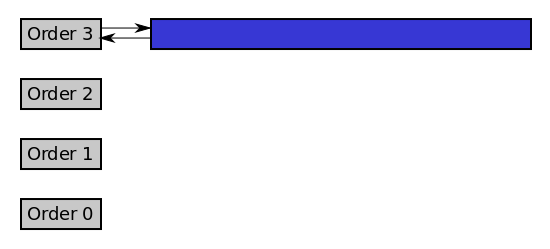
\includegraphics[width=0.7\textwidth]{buddy_alloc0.png}
\end{center}
\begin{itemize}
  \item Для примера ограничемся только порядками от 0 до 3;
  \item допустим вся память описывается блоком порядка 3:
  \begin{itemize}
    \item начальная конфигурация может состоять из нескольких блоков;
  \end{itemize}
  \item будем алоцировать блоки порядка 0:
  \begin{itemize}
    \item можно алоцировать блоки произвольного порядка.
  \end{itemize}
\end{itemize}
\end{frame}

\begin{frame}
\frametitle{Алокация 2/3}
\begin{center}
  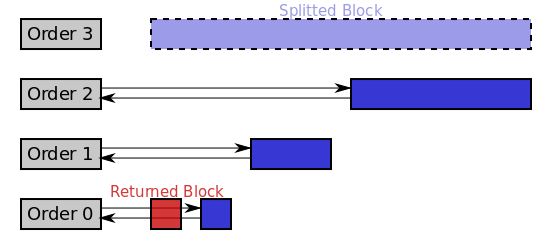
\includegraphics[width=0.7\textwidth]{buddy_alloc1.png}
\end{center}
\begin{itemize}
  \item Список с блоками нужного размера может быть пуст
  \begin{itemize}
    \item можем взять блок большего размера и разбить его;
  \end{itemize}
  \item делим блок пока не останется блок нужного размера:
  \begin{itemize}
    \item ненужную половину добавляем в соответствующий список.
  \end{itemize}
\end{itemize}
\end{frame}

\begin{frame}
\frametitle{Алокация 3/3}
\begin{center}
  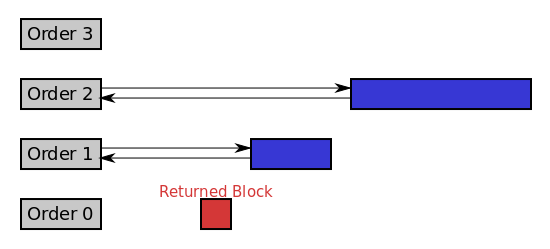
\includegraphics[width=0.7\textwidth]{buddy_alloc2.png}
\end{center}
\begin{center}
  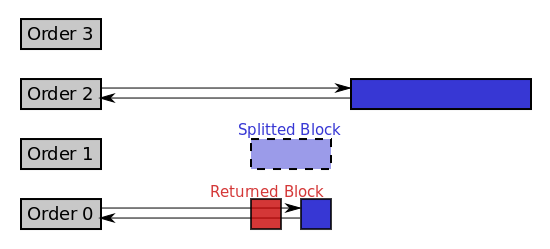
\includegraphics[width=0.7\textwidth]{buddy_alloc3.png}
\end{center}
\end{frame}

\begin{frame}
\frametitle{Освобождение 1/2}
\begin{center}
  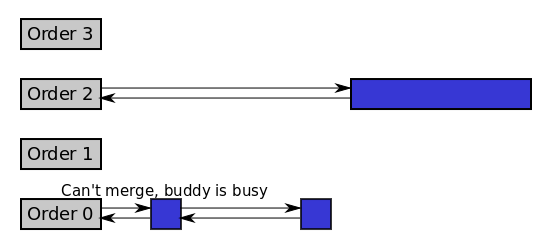
\includegraphics[width=0.7\textwidth]{buddy_free0.png}
\end{center}
\begin{itemize}
  \item При освобождении блок добавляется в соответствующий список
  \begin{itemize}
    \item при освобождении нужно проверить свободен ли buddy блок.
  \end{itemize}
\end{itemize}
\end{frame}

\begin{frame}
\frametitle{Освобождение 2/2}
\begin{center}
  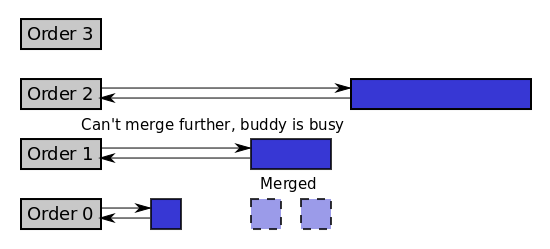
\includegraphics[width=0.7\textwidth]{buddy_free1.png}
\end{center}
\begin{itemize}
  \item Если buddy блок свободен, то можно блоки можно вновь объединить
  \begin{itemize}
    \item для объединенного блока также нужно проверить buddy блок.
  \end{itemize}
\end{itemize}
\end{frame}

\begin{frame}
\frametitle{Дескрипторы регионов}
\begin{itemize}
  \item Для блоков нам необходимо уметь:
  \begin{itemize}
    \item определять свободен блок или нет;
    \item уметь связать блоки в список;
  \end{itemize}
  \item заведем дескриптор для каждого региона размера \emph{PAGE\_SIZE}:
  \begin{itemize}
    \item дескрипторы можно связывать в список (хранят \emph{prev} и
    \emph{next});
  \end{itemize}
  \item дескриптор первого региона блока - представитель блока:
  \begin{itemize}
    \item в нем хранится признак свободности/занятости;
    \item порядок блока, представителем которого он является;
    \item блок порядка $i$ свободен, если \emph{представитель свободен и
    порядок представителя равен $i$}.
  \end{itemize}
\end{itemize}
\end{frame}

\begin{frame}
\frametitle{Проблема курицы и яйца}
\begin{itemize}
  \item Где брать память под дескрипторы?
  \begin{itemize}
    \item алоцировать фиксированное заранее количество дескрипторов
    \begin{itemize}
      \item возможно придется алоцировать с большим запасом;
    \end{itemize}
    \item использовать другой алокатор памяти, чтобы алоцировать дескрипторы
    \begin{itemize}
      \item например, описанный ранее алгоритм или более простой;
      \item нам не нужно освобождение, чтобы инициализировать Buddy алокатор.
    \end{itemize}
  \end{itemize}
\end{itemize}
\end{frame}
